\section{Procedure}
\label{sec:procedure}

The used diode laser in this experiment provides a beam with an output power of up to $\SI{70}{\milli\watt}$
and a wavelength around $\SI{785}{\nano\meter}$, almost ideal for examining rubidium transitions.

\subsection{Experimental setup}

The schematic experimental setup is illustrated in Fig. \ref{fig:setup}.
On the right side one can view the diode laser with the diffraction grating producing the laser beam.
The diffraction grating has two adjustable angles, the horizontal one to vary the highest gain wavelength and the vertical
one to vary the external cavity length.
The beam is splitted at the 50/50 beam splitter so that one part proceeds directly to a photo diode, where
its intensity is estimated, and the other part hits the Rubidium cell. A CCD infrared camera is mounted next to the cell
to view the fluorescence, when the right beam wavelength is adjusted. The remaining intensity of the laser beam
after passing the cell is again detected by a photo diode.

\begin{figure}
  \centering
  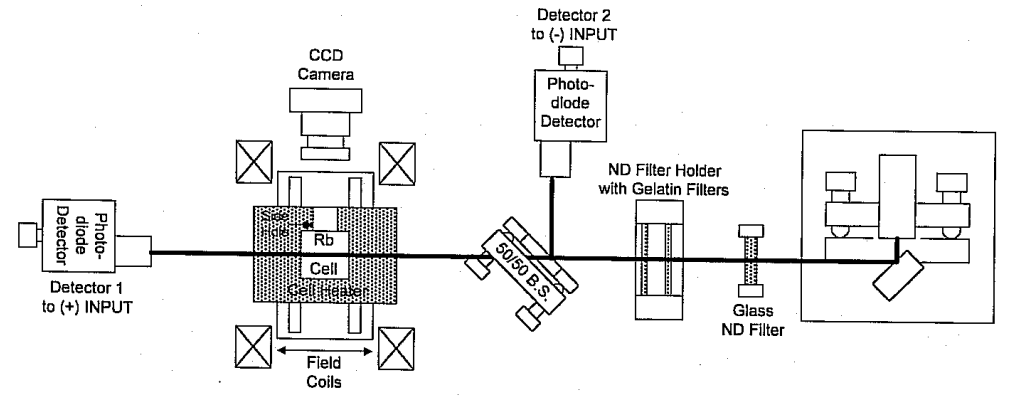
\includegraphics[height=5cm]{Ordnername/setup.png}
  \caption{Schematic experimental setup to monitor the Rubidium spectrum \cite{manual}.}
  \label{fig:setup}
\end{figure}

\subsection{Adjusting steps}

The full experimental procedure deals with the adjusting of the laser. The step by step
manual can be viewed in source \cite{manual}. To start with the experiment the Rubidium cell temperature
is adjusted to $\SI{50}{\celsius}$ and the wiring between diode laser and laser controller is checked.

The first important step is the estimation of the threshold current. Therefor
the output beam is absorbed by an infrared screen and monitored by the camera.
One varies the current, so that a typical speckle pattern only just can be viewed.
After that one varies the current and the angles of the diffraction grating alternating
to estimate the threshold current as exact as possible.

The second step is the adjusting of the laser to observe the Rubidium fluorescence.
Therefor the camera is mounted like shown in Fig. \ref{fig:setup} and the ramp generator
and the piezo module are connected to the setup. The angles of the diffraction grating are
again varied until one sees the fluorescence on the monitor.

For the last step the entire setup presented in Fig. \ref{fig:setup} is needed.
By using the detector electronics the two signals detected by the photodiodes are
substracted. To get succesfull results one may has to modify the altitude and the position of the
photodiodes. With the help of the piezo module one can view a continuous
Doppler broaden spectrum on the oscilloscope screen.
